\chapter{Implementazione}\label{implementazione}

In questo capitolo viene descritto il processo di implementazione della soluzione proposta per la valutazione di sistemi distribuiti. L'obiettivo principale è illustrare i dettagli dell'infrastruttura creata, i componenti utilizzati e il funzionamento generale del sistema. \\
La prima parte si concentra sul \emph{target} dell'assurance, ovvero l'ambito dei servizi e delle applicazioni monitorati.
Successivamente, si descrive l'\emph{infrastruttura sperimentale} utilizzata per il deployment basata su MicroK8s.
La parte centrale del capitolo si focalizza sul deployment e sul funzionamento dello \emph{stack} fornito da \emph{Elasticsearch}.
Infine si tratta l'\emph{Assurance Engine}, ovvero il framework di monitoring in corso di sviluppo.

\section{Assurance Target}
Il sistema implementato ha come \textit{scope}, ovvero obbiettivo di monitoring, una determinata tipologia di servizi, concentrandosi su applicazioni o \gls{VM} containerizzate e deployate all'interno del cluster Kubernetes del laboratorio. In altre parole, il target del sistema sono esclusivamente entità (applicazioni o \gls{VM}) distribuite internamente al cluster, che possono presentare una struttura centralizzata o distribuita.
Le entità classificabili come possibili esempi di target vanno dai generici servizio deployabili in un cluster kubernetes come un web server o un database ad entità più specifiche come il servizio di GitLab\footnote{\url{https://about.gitlab.com/}} fino ad arrivare a sistemi operativi completamente deployati (\gls{VM}) sul cluster tramite l'utilizzo di KubeVirt\footnote{\url{https://kubevirt.io/}}.

Una delle caratteristiche più rilevanti di questo sistema è la capacità di monitorare sia entità predisposte al monitoring trasparente, sia entità che richiedono l'ausilio di agenti per il monitoraggio, come descritto nella Sezione \ref{estrazione inforamzioni}.
La flessibilità di questo approccio permette di superare un'importante limitazione del monitoring, consentendo la raccolta di dati da entità distribuite eseguite in container, pur non avendo un controllo diretto sul loro funzionamento in quanto si tratta di servizi o applicazioni prodotti da enti terze, ``pronti all'uso'' e con un'interfaccia di tipo \textit{black-box}.
Il sistema è quindi in grado di monitorare ogni tipo di applicativo distribuito all'interno del cluster. Questa integrazione è ulteriormente facilitata dalle \emph{integrazioni} native che \emph{Elasticsearch} mette a disposizione per interfacciarsi con vari servizi o applicativi standard, come Kubernetes o servizi offerti da Apache e \gls{AWS}, ecc.

\section{Experimental setup}
In questa sezione verrà descritto l'ambiente Kubernetes utilizzato per l'implementazione e lo sviluppo del sistema, con un'analisi delle sue configurazioni e componenti principali.

Il cluster è stato sviluppato tramite \textbf{MicroK8s}\footnote{\url{https://microk8s.io/}}, una distribuzione \textit{lightweight} di Kubernetes sviluppata da Canonical\footnote{\url{https://canonical.com/}} e progettata per essere facilmente installabile ed eseguibile.
MicroK8s è caratterizzato da un'architettura modulare che consente agli utenti di attivare solo i componenti necessari per il proprio ambiente.
L'installazione predefinita include un cluster Kubernetes completamente funzionante, con l'opzione di aggiungere delle componenti (add-ons) come DNS, ingress, dashboard, e altri servizi comuni tramite semplici comandi.
Fornisce quindi un cluster Kubernetes facilmente componibile.
Il pacchetto include anche il supporto per il deployment di cluster distribuiti, noti anche come cluster multi-nodo. \\
L'infrastruttura sperimentale è quindi costituita da un cluster Kubernetes deployato tramite MicroK8s su 3 nodi fisici eterogenei presenti nel laboratorio, ognuno dei quali possiede differenti capacità in termini computazionali e di storage.
Nella Tabella~\ref{risorse nodi} vengono indicate le specifiche di ogni nodo presente, in questo modo l'architettura del sistema diventa replicabile permettendo l'esecuzione di esperimenti su un setup identico.

%https://tex.stackexchange.com/questions/60601/evenly-distributing-column-widths

%\textbf{CPU Core} & \textbf{Frequenze}
\begin{table}[h!]
	\caption{Risorse disponibili nel sistema}\label{risorse nodi}
	\centering
	\begin{tabularx} {\textwidth}
		{c*{6}{C}} % C è un column type definiti nel main
		\toprule
		\multirow{2}{*}{\textbf{Nodo}} & \multicolumn{3}{c}{\textbf{CPU}} & \multirow{2}{*}{\textbf{RAM}} & \multirow{2}{*}{\textbf{Disco}}                                                     \\

		\cmidrule(r){2-4} %permette di estendere solo sotto alcune colonne definite multi column
		                               & \textbf{Modello}                 & \textbf{Core}                 & \textbf{Frequenza}                                                                  \\
		\midrule
		balthasar                      & Broadwell                        & 16                            & 2.10 GHz                        & 15.6 GiB                 & 296.8 GiB                \\
		casper                         & Broadwell                        & 16                            & 2.10 GHz                        & 23.4 GiB                 & 296.8 GiB                \\
		\multirow{2}{*}{melchior}      & \multirow{2}{*}{EPYC 7453}       & 28                            & 2.75 GHz                        & \multirow{2}{*}{252 GiB} & \multirow{2}{*}{1.7 TiB} \\
		                               &                                  & 28                            & 2.75 GHz                        &                         &                         \\

		\bottomrule
		Totale                         &                                  & 88                            &                                 & 291 GiB                 & 2.3 TiB                  \\
		\bottomrule
	\end{tabularx}
\end{table}

Per la gestione dello \textbf{storage distribuito}, il cluster utilizza Longhorn\footnote{\url{https://longhorn.io/}}, un un sistema di storage a blocchi distribuito (\textit{distributed block storage system}) e \textit{open-source}.
Fornisce \emph{volumi persistenti} altamente disponibili e affidabili attraverso la loro \emph{replica} archiviata su più nodi, assicurando così la continuità del servizio anche in caso di failure hardware o di rete (no \textit{single-point-of-failure}).
Grazie alla sua architettura leggera e all'integrazione nativa con Kubernetes, Longhorn semplifica la gestione dello storage dinamico e scalabile, supportando operazioni come il provisioning automatico dei volumi.
Una delle caratteristiche chiave offerte da Longhorn sono le funzionalità di \emph{backup} e \emph{snapshot} \emph{incrementali}, facilmente gestibili attraverso la sua interfaccia utente.
Le snapshot consentono di catturare lo stato dei volumi in determinati momenti nel tempo, facilitando il ripristino rapido dei dati in caso di errori o corruzione (system side) o per la creazione di repliche.
I backup, invece, permettono di salvare copie dei dati su storage esterni al cluster basandosi sugli snapshot, aumentando ulteriormente la sicurezza e la durabilità delle informazioni critiche (user side).
Queste funzionalità contribuiscono a garantire l'integrità e la disponibilità dei dati del \textit{persistent volume storage} sia all'interno che all'esterno del cluster Kubernetes, supportando strategie di disaster recovery efficaci e riducendo il rischio di perdita di dati.

Il cluster utilizza anche un plugin \textbf{\gls{CNI}}, che si occupa di configurare dinamicamente le risorse di rete e rimuoverle dai container terminati, per gestire il networking interno.
Il plugin installato è Kube-ovn\footnote{\url{https://www.kube-ovn.io/}}, una soluzione avanzata e performante che combina le capacità di Kubernetes con le ricche e comprovate funzionalità di virtualizzazione di rete basate su \gls{OVN}\footnote{\url{https://www.ovn.org/}}, una piattaforma per il \gls{SDN}, in un ambiente \textit{cloud-native}; consente la creazione di reti logiche e virtuali che si sovrappongono all'infrastruttura fisica esistente.
\gls{OVN} si costituisce come una serie di \textit{daemon} per \textit{Open vSwitch}\footnote{\url{https://www.openvswitch.org/}} che traducono le configurazioni di rete virtuale in \textit{OpenFlow}, un protocollo di comunicazione che permette la gestione del flusso di dati all'interno di switch e router in reti software-defined.
Fornisce quindi un maggiore controllo sullo switching/routing dei pacchetti nella rete e sul binding delle porte logiche. Consente inoltre la specifica di policy di sicurezza avanzate (Firewall) e un controllo completo sulla rete (\textit{load-balancing, Quality of Service, monitoring}).
L'approccio \gls{SDN} consente una gestione delle reti che separa il \textit{control plane} della rete, la logica che decide la topologia di rete e le informazioni nelle routing tables, dal \textit{data-plane}, che si occupa dell'effettivo inoltro del traffico, consentendo una gestione programmabile e centralizzata della rete, la quale diventa più flessibile e dinamica adattandosi alle esigenze.


Il cluster di riferimento gestisce tutte le entità, siano esse servizi o \gls{VM}, come risorse di calcolo e storage creando uno strato di astrazione al di sopra di esse che consente di generalizzarne l'aspetto. Questa infrastruttura distribuita su vari nodi e con componenti eterogenee rappresenta uno scenario ideale per \textbf{test realistici}, grazie alla sua capacità di rispecchiare ambienti applicativi complessi e variabili.

\section{ECK Stack}
La prima fase dell'implementazione è costituita dal deployment dello stack \gls{ECK}\footnote{\url{https://artifacthub.io/packages/helm/elastic/eck-stack}} che estende le funzionalità di orchestrazione di base di Kubernetes per supportare la configurazione e la gestione di Elasticsearch, Kibana, Elastic Agent, Fleet Server, ecc.
Segue un'illustrazione delle varie componenti deployate.

\paragraph{Elasticsearch}
il cuore dello stack Elastic, è un archivio dati scalabile e distribuito con implementato un motore di ricerca e analisi utilizzabile tramite query presso le \gls{API} RESTful che espone. La sua architettura distribuita permette di scalare orizzontalmente, distribuendo il carico di lavoro su più nodi, garantendo così elevata disponibilità e prestazioni.
Viene utilizzato per cercare, indicizzare, archiviare e analizzare dati di tutte le forme in tempo reale date le ottimizzazioni in termini di performance.

\paragraph{Kibana}
è la \gls{GUI} progettata per \emph{visualizzare e osservare}, \emph{cercare}, \emph{analizzare} e \emph{gestire} i dati archiviati in Elasticsearch. Fornisce strumenti per creare dashboard, grafici, tabelle e mappe interattive, eseguire ricerche avanzate e monitorare in tempo reale i dati.

\paragraph{Elastic Agent}
rappresentano una singola e unificata modalità per aggiungere monitoring per log, metriche e altri tipi di dati a un host, semplificando e velocizzando l'implementazione nell'intera infrastruttura. Forniscono anche funzionalità di protezione dell'host da minacce di sicurezza.
Elastic fornisce delle \emph{Integration} per gli agent, ovvero una raccolta di asset che definiscono come collegarsi ad uno specifico prodotto o servizio esterno attraverso lo Stack Elastic, raccogliendo, archiviando e visualizzando facilmente qualsiasi dato da qualsiasi fonte. Forniscono inoltre risorse pronte all'uso come dashboard, visualizzazioni e pipeline per estrarre campi strutturati da log ed eventi provenienti da questi servizi.
Infine, ogni agente ha una singola policy che può essere aggiornata per aggiungere integrazioni per nuove fonti di dati e protezioni di sicurezza.

\paragraph{Fleet}
è un componente che fornisce gestione centralizzata degli Elastic Agent e delle relative policy attraverso una specifica interfaccia utente di Kibana.
Fleet funge da canale di comunicazione per gli Elastic Agent, i quali effettuano regolarmente il \textit{check-in} per aggiornamenti e comunicando il relativo stato di salute. Quando viene apportata una modifica a una policy o ad una integrazione, tutti gli agenti ricevono l'aggiornamento durante il \textit{check-in} successivo senza necessità di intervento manuale.

\subsection{Deployment}
Lo stack è reso disponibile tramite Helm\footnote{\url{https://helm.sh/}}, un package-manager per Kubernetes che semplifica la definizione, l'installazione, l'upgrade e la gestione di applicazioni su un cluster. Si basa su \emph{chart}, pacchetti preconfigurati di risorse Kubernetes che permettono di automatizzare e standardizzare il deployment di applicazioni, riducendo la complessità e migliorando la consistenza tra ambienti.
Gli \emph{helm chart} da deployare sono tre: \texttt{eck-operator}\footnote{\url{https://artifacthub.io/packages/helm/elastic/eck-operator}}, \texttt{eck-stack}\footnote{\url{https://artifacthub.io/packages/helm/elastic/eck-stack}} e \texttt{kube-state-metrics}\footnote{\url{https://artifacthub.io/packages/helm/bitnami/kube-state-metrics}}.

\paragraph{eck-operator}
è il componente che si occupa di automatizzare il deployment, la gestione e l'orchestrazione di tutto lo stack \gls{ECK} e quindi, nel nostro contesto, di Elasticsearch, Kibana e degli Elastic Agent.
Il deployment non prevede configurazioni particolari e può essere fatto attraverso: \texttt{helm install my-eck-operator elastic/eck-operator}

\paragraph{eck-stack}
è il chart che contiene tutti i componenti deployabili dello stack;
si pone come l'aggregazione di 6 chart corrispondenti ai 6 applicativi offerti. Nel dettaglio sono eck-elasticsearch, eck-kibana, eck-agent, eck-fleet-server, eck-logstash ed infine eck-apm-server. \\
La configurazione di default abilita solo Elasticsearch e Kibana, in quanto servizi esistenziali dello stack, ma per il nostro caso di studio dovranno essere abilitati anche gli Agent e il Fleet Server.
Dopo aver selezionato i servizi da deployare è necessario andare a configurare singolarmente ciascuno di essi, andando ad impostare opportunamente i \textit{values} offerti dal relativo chart.

\paragraph{kube-state-metrics}
è un semplice servizio che ascolta il server \gls{API} di Kubernetes e, senza modifiche, genera metriche sullo stato degli oggetti, concentrandosi sulla salute dei vari oggetti interni al cluster come nodi, deployment e pod; riflette lo \emph{stato corrente del cluster} ed è utilizzato per monitorarlo.
A differenza di \emph{kubectl}, che applica certe euristiche ai dati, restituisce i dati grezzi, così come vengono ritornati dalle \gls{API} di kubernetes.
Si tratta di un sistema di monitoring di tipo Pull in quanto va ad esporre le metriche che collezione, come plain-text, su un endpoint HTTP, al \emph{path:} \emph{/metrics} sulla porta \emph{8080}.
Gli endpoint verranno interrogati dagli Agent per collezionarne i dati. \\
Il deployment non prevede configurazioni particolari e può essere fatto attraverso: \texttt{helm install my-kube-state-metrics bitnami/kube-state-metrics --version 4.2.12}

\subsection{ECK-stack deployment values}
In questa sezione verranno forniti e discussi i \textit{values} utilizzati per la configurazione del Helm \texttt{eck-stack}.

\paragraph{Elasticsearch}
In questa configurazione illustrata nel Codice \ref{elasticsearch values} viene specificata l'abilitazione e il nome da assegnare ai componenti che verranno deployati, successivamente viene specificata la struttura dei nodi.
\begin{lstlisting}[language=yaml, caption= Elasticsearch yaml values \label{elasticsearch values}, basicstyle=\ttfamily]
  eck-elasticsearch:
    enabled: true
    fullnameOverride: elasticsearch
    nodeSets:
      - config:
          node.store.allow_mmap: false
        count: 3
        name: default

\end{lstlisting}

\paragraph{Kibana}
Le specifiche di Kibana possiamo vederle come suddivise in due parti.
La prima, visibile nel Codice \ref{kibana values}, riguarda il servizio di Kibana vero e proprio specificandone l'abilitazione, il nome da assegnare al componente deployato e delle specifiche riguardanti il numero di repliche da creare e il riferimento ad Elasticsearch. Vengono infine specificate delle configurazioni riguardanti gli endpoint su cui si trovano il servizio di Elasticsearch e il Fleet Server.

\begin{lstlisting}[language=yaml, caption= Kibana yaml values \label{kibana values}, basicstyle=\ttfamily]
  eck-kibana:
    enabled: true
    fullnameOverride: kibana
    spec:
      count: 1
      elasticsearchRef:
        name: elasticsearch
      config:
        xpack.fleet.agents.elasticsearch.hosts:
          ["https://elasticsearch-es-http.elastic-stack.svc:9200"]
        xpack.fleet.agents.fleet_server.hosts:
          ["https://fleet-server-agent-http.elastic-stack.svc:8220"]
\end{lstlisting}

La seconda, visibile nel Codice \ref{kibana policy values}, invece, si focalizza sul fornire delle configurazioni per le policy che il Fleet Server (\texttt{id: eck-fleet-server}) e gli Agent (\texttt{id: eck-agent}) dovranno implementare. Le policy qui definite verranno utilizzate come values nella configurazione dei campi policyID dei chart \texttt{eck-agent} ed \texttt{eck-fleet-server}.

\begin{lstlisting}[language=yaml, caption= Kibana Policy yaml values \label{kibana policy values}, basicstyle=\ttfamily]
spec:
  config:
    xpack.fleet.agentPolicies:
    - name: Fleet Server on ECK policy
      id: eck-fleet-server
      namespace: default
      monitoring_enabled:
      - logs
      - metrics
      package_policies:
      - name: fleet_server-1
        id: fleet_server-1
        package:
          name: fleet_server
    - name: Elastic Agent on ECK policy
      id: eck-agent
      namespace: default
      monitoring_enabled:
      - logs
      - metrics
      unenroll_timeout: 900
      package_policies:
      - package:
          name: system
        name: system-1
      - package:
          name: kubernetes
        name: kubernetes-1
\end{lstlisting}


\paragraph{Elastic Agent}
In questa configurazione, illustrata nel Codice \ref{agent values}, viene specificata l'abilitazione e delle specifiche dei singoli agent come la policy che devono seguire (definita nelle configurazioni di kibana), il riferimento a Kibana, che fornisce automaticamente quello di Elasticsearch senza specificarlo, e infine il riferimento al Fleet Server con la relativa modalità di esecuzione degli agenti \textit{fleet-managed} (contrariamente alla modalità \textit{stand-alone})
\begin{lstlisting}[language=yaml, caption= Elastic Agent yaml values \label{agent values}, basicstyle=\ttfamily]
  eck-agent:
    enabled: true
    spec:
      policyID: eck-agent
      kibanaRef:
        name: kibana
      elasticsearchRefs: []
      fleetServerRef:
        name: fleet-server
      mode: fleet
\end{lstlisting}

\paragraph{Fleet server}
Configurazione molto semplice, visibile nel Codice \ref{fleet values}, in cui viene specificata l'abilitazione, il nome da assegnare al componente deployato e delle specifiche riguardanti la policy da assegnare al server (definita nelle specifiche di Kibana) e i riferimenti a Kibana ed Elasticsearch
\begin{lstlisting}[language=yaml, caption= Fleet Server yaml values \label{fleet values}, basicstyle=\ttfamily]
  eck-fleet-server:
    enabled: true
    fullnameOverride: "fleet-server"
    spec:
      policyID: eck-fleet-server
      kibanaRef:
        name: kibana
      elasticsearchRefs:
      - name: elasticsearch
\end{lstlisting}

\subsection{Funzionamento}
La Figura \ref{eck flow} mostra il flusso di esecuzione di \gls{ECK} numerando le attività dalla 1 alla 8. Il flusso verrà percorso durante la seguente spiegazione.

\begin{figure}[ht]
	\centering
	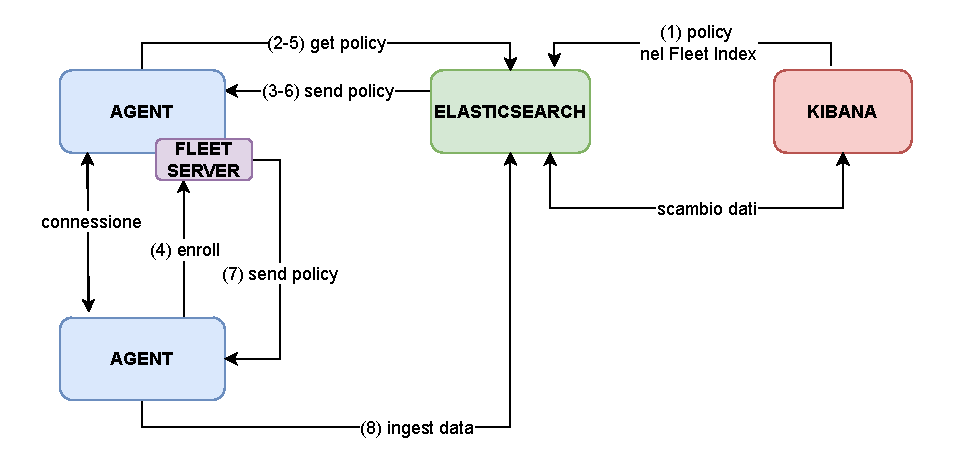
\includegraphics[width=1\linewidth]{images/ECK_flow.drawio.pdf}
	\caption{Diagramma del flusso di funzionamento dello stack}\label{eck flow}
\end{figure}

All'avvio di \emph{Kibana} le policy specificate nella configurazione, avvenuta tramite \emph{helm chart}, vengono salvate in un indice, denominato \emph{Fleet}, all'interno di Elasticsearch. \\
Il \emph{Fleet Server}, all'avvio, stabilisce una connessione tramite i riferimenti posti tra i values con Kibana, per abilitare l'interfaccia grafica di gestione Fleet, e con Elasticsearch per ottenere i dati contenuti nell'indice di Fleet, ovvero le policy definite. In concreto, il Fleet Server funziona come un agente normale, con la differenza che viene ``enrollato'' in una policy server.\\
Gli \emph{Agenti}, all'avvio, essendo \textit{fleet-enrolled} cercheranno di stabilire una connessione con il Fleet Server tramite il riferimento specificato.\@ Andranno a richiedere al server la policy specificata nella loro configurazione (\texttt{policyID: eck-agent}) e Fleet si occuperà di recuperarla dall'indice di Elasticsearch per consegnarla al richiedente legittimo. Si dice quindi terminata la fase di \emph{enrollment}. \\
Aprendo l'interfaccia di Fleet tramite Kibana è quindi possibile gestire le due policy caricate e i relativi agent che sono stati ``enrollati''; le modifiche effettuate tramite il Fleet server alle policy vengono riflesse nell'indice di Elasticsearch e negli agent che seguono quella policy, effettuando un upgrade automatico.
Viene mantenuta una connessione attiva tra agenti e fleet server per controllare lo stato di salute e la disponibilità di aggiornamenti; quando un agente si collega e c'è stato un cambiamento, il Fleet Server recupera da Elasticsearch la policy e la consegna all'agente effettuando così un aggiornamento autonomo. \\
Una volta che l'intera infrastruttura è stata deployata si hanno 3 agenti \emph{fleet-enrolled}, uno per ciascuno nodo, che vanno ad usare le informazioni contenute nella policy per raccogliere i dati e inviarli ad Elasticsearch; gli agenti hanno un'architettura di tipo Push in quanto inviano attivamente i dati ad un endpoint che si occuperà di salvarli in appositi indici.\\
Tramite l'interfaccia di gestione delle policy è possibile scegliere quali Integrazioni aggiungere, andando così a raccogliere dati da una nuova sorgente e causando un rilascio di una nuova versione della rispettiva policy con conseguente aggiornamento degli agent. \\
Oltre a svolgere operazioni di ricerca e analisi tramite la \gls{GUI} di Kibana è possibile inviare query agli endpoint di Elasticsearch, i quali mettono a disposizione una serie di \gls{API} REST\footnote{\url{https://www.elastic.co/guide/en/elasticsearch/reference/current/rest-apis.html}}.

\section{Assurance Engine}
L'applicativo viene sviluppato in Rust\footnote{\url{https://www.rust-lang.org/}}, un linguaggio sicuro e ad alte prestazioni che previene molti errori comuni, fondandosi su 3 pacchetti principali quali Tokio\footnote{\url{https://tokio.rs/}}, per la gestione dell'esecuzione asincrona, Poem\footnote{\url{https://crates.io/crates/poem}}, come framework web, e PoemOpenAPI\footnote{\url{https://crates.io/crates/poem-openapi}}, per l'implementazione automatica di \gls{API} e della relativa documentazione. \\
L'engine sviluppato si basa inoltre sui due concetti principali dell'Assurance Methodology, le \textbf{metriche} e i \textbf{contratti}, visti nella Sezione \ref{assurance methodology} e ora realizzati concretamente sotto forma di \emph{Trait}; un componente Rust che definisce in modo astratto il comportamento/la funzionalità che un particolare tipo ha e può condividere con altri tipi.  \\
La Figura \ref{metriche_contratti} mostra uno schema che, partendo dai dati grezzi, illustra i passaggi chiave da compiere prima di arrivare ad un report del sistema.

\begin{figure}[ht]
	\centering
	
\includegraphics[width=.9\linewidth]{images/ae/metriche-contratti.drawio.pdf}
	\caption{Diagramma del funzionamento}\label{metriche_contratti}
\end{figure}

Le funzionalità sviluppate vengono poi rese accessibili tramite l'esposizione di \textbf{\gls{API} rest} conformate ai criteri di \emph{OpenAPI Specification v3}\footnote{\url{https://github.com/OAI/OpenAPI-Specification/blob/main/versions/3.1.0.md}}; vengono quindi seguite alcune delle linee standard precedentemente identificate nella Sezione \ref{standard}. \\
Segue l'illustrazione dei vari punti chiave nominati.


\subsection{Metric e Measurement}\label{metric trait}
\'E stato definito il trait parametrico \texttt{Metric} come riportato nel Codice \ref{trait metric} che permette di specificare il tipo dell'argomento (\texttt{Arguments}) e dell'\texttt{Output}, i quali devono a loro volta soddisfare determinati \emph{trait bounds} (Send + Sync + \dots). Fornisce quindi un'interfaccia generica che codifica la struttura di una metrica definendo la firma di due metodi, \texttt{description()} e \texttt{measure()}.
Il primo è semplicemente una funzione che ritorna una descrizione letterale della metrica. Il secondo, invece, è il metodo che concretamente va ad ottenere le misurazioni dagli endpoint di monitoring.

\begin{lstlisting}[language=Rust, caption= Metric Trait \label{trait metric}, basicstyle=\ttfamily ]
  #[async_trait]
  pub trait Metric<Arguments, Output>
      where
    Arguments: Send + Sync + Type + ParseFromJSON + ToJSON,
    Output: Send + Sync + Type + ParseFromJSON + ToJSON,
  {
      fn id(&self) -> Box<str> {
          Box::from(std::any::type_name::<Self>())
      }

      fn description(&self) -> Box<str>;

      async fn measure(&self, args: Arguments)
        -> Result<Measurement<Arguments, Output>, Error>;
  }
\end{lstlisting}

L'implementazione concreta, in questo contesto, di quest'ultimo metodo va a costruire ed eseguire le query contro le \gls{API} esposte dal servizio di Elasticsearch (endpoint) per ottenere i dati (\textit{evidence}).
Prende come input un argomento, \textit{args}, del tipo generico da definire, \texttt{Arguments}, ovvero una struttura specifica che contiene tutti gli argomenti necessari a configurare la richiesta, include quindi sia la query vera e propria che dei parametri di configurazione come l'indice di interesse e la dimensione, come rappresentato nel Codice \ref{Arguments struct}.

\begin{lstlisting}[language=Rust, caption= Arguments Struct \label{Arguments struct}, basicstyle=\ttfamily ]
  #[derive(Debug, Clone, PartialEq, serde::Deserialize,
      serde::Serialize, Object)]
  pub struct BasicSearchArgs {
      pub query: Value,
      pub index: Vec<String>,
      pub from: Option<i64>,
      pub size: Option<i64>,
  }
\end{lstlisting}

\subsubsection{Measurement}\label{measurement section}
In output, a meno di errori, il metodo \texttt{measure()} restituisce un \texttt{Measurement}, una struttura che rappresenta il risultato dalla misurazione, costituita dai campi \texttt{time}, \texttt{args} e \texttt{value} come mostrato nel Codice \ref{Measurement struct}.
Rispettivamente contengono l'istante di tempo in cui è avvenuta la misurazione, gli argomenti passati come input (\texttt{args} di tipo \texttt{Arguments}) e i valori ottenuti.

\begin{lstlisting}[language=Rust, caption= Measurement Struct \label{Measurement struct}, basicstyle=\ttfamily ]
  #[derive(Object)]
  pub struct Measurement<Arguments, Output>
      where
    Arguments: Send + Sync + Type + ParseFromJSON + ToJSON,
    Output: Send + Sync + Type + ParseFromJSON + ToJSON,
  {
      /// Time instant of measurement
      pub time: OffsetDateTime,
      /// Arguments in input
      pub args: Arguments,
      /// Value registered
      pub value: Output,
  }
\end{lstlisting}

Qui entra in gioco il secondo parametro di tipo generico da definire, ovvero \texttt{Output}, che definisce la struttura del risultato da andare ad includere all'interno del \texttt{Measurement}, come si può vedere nel Codice \ref{Output struct} si tratta di un solo valore, \texttt{output}, che permette il contenimento di una stringa in formato json.

\begin{lstlisting}[language=Rust, caption= Output Struct \label{Output struct}, basicstyle=\ttfamily ]
  #[derive(Debug, Clone, PartialEq, serde::Deserialize,
      serde::Serialize, Object)]
  pub struct BasicSearchOutput {
      pub output: Value,
  }
\end{lstlisting}

\subsection{Contract ed Evaluation}\label{contract section}
\'E stato definito il trait parametrico \texttt{Contract} come riportato nel Codice \ref{trait contract} che permette di specificare il tipo dell'argomento (\texttt{Arguments}), il quale deve a sua volta soddisfare determinati \textit{trait bounds}. Fornisce quindi un'interfaccia generica che codifica la struttura di un contratto definendo la firma di due metodi, \texttt{description()} e \texttt{evaluate()}. Il primo, come per le metriche, è semplicemente una funzione che ritorna una descrizione letterale. Il secondo, invece, è il metodo che concretamente valuta le misurazioni raccolte combinando strutture di condizioni booleane.

\begin{lstlisting}[language=Rust, caption= Contract Trait \label{trait contract}, basicstyle=\ttfamily ]
  #[async_trait]
  pub trait Contract<Arguments>
      where
    Arguments: Send + Sync + Type + ParseFromJSON + ToJSON,
  {
      fn id(&self) -> Box<str> {
          Box::from(std::any::type_name::<Self>())
      }

      fn description(&self) -> Box<str>;

      async fn evaluate(&self, args: Arguments)
        -> Result<Evaluation<Arguments>, Error>;
  }
\end{lstlisting}

L'implementazione concreta, in questo contesto, di quest'ultimo metodo va ad eseguire il metodo \texttt{measure()}, definito con l'implementazione del \emph{trait metric} visto sopra, e a svolgere dei controlli sulle \emph{misurazioni} che ottiene andando a verificare il superamento o meno di specifiche valutazioni, restituendo un valore booleano che ne definisce l'esito finale.
Prende come input un argomento, \texttt{args}, del tipo generico da definire,
\texttt{Arguments}, ovvero una struttura specifica i cui campi contengono dei valori di riferimento da confrontare con i valori delle misurazioni, per valutare il soddisfacimento o meno del contratto. Si potrebbero impostare, per esempio, dei valori che si desiderano di temperatura minimi, medi e massimi per poi controllare se le misurazioni ottenute rispettano i criteri specificati.
Nel Codice \ref{argument contract struct} viene rappresentata la ''struttura tipo''.

\begin{lstlisting}[language=Rust, caption= Argument Contract Struct\label{argument contract struct}, basicstyle=\ttfamily ]
  #[derive(Debug, Clone, PartialEq, Serialize,
     Deserialize, Object)]
  pub struct SearchContractArgs {
    //values to check the fields with
  }
\end{lstlisting}

\subsubsection{Evaluation}\label{evaluation section}
In output, a meno di errori, il metodo \texttt{evaluate} restituisce un \texttt{Evaluation}, una struttura che rappresenta il risultato della valutazione, costituita dai campi \texttt{time}, \texttt{args} e \texttt{value} come mostrato nel Codice \ref{Evaluation struct}. Rispettivamente contengono l'istante di tempo in cui è avvenuta la misurazione, gli argomenti passati come input (\textit{args} di tipo \texttt{Arguments}) e il valore booleano ottenuto.

\begin{lstlisting}[language=Rust, caption= Evaluation Struct \label{Evaluation struct}, basicstyle=\ttfamily ]
  #[derive(Debug, Clone, PartialEq, Serialize, Deserialize)]
  pub struct Evaluation<Arguments>
      where
    Arguments: Send + Sync + Type + ParseFromJSON + ToJSON,
  {
      /// Time entry in input
      pub time: OffsetDateTime,
      /// Arguments in input
      pub args: Arguments,
      /// Value verified as valid
      pub value: bool,
  }
\end{lstlisting}

\subsection{API}
Come accennato prima le \gls{API} vengono implementate attraverso il crate PoemOpenAPI, il quale garantisce che se il codice compila correttamente allora è pienamente conforme alle Specifiche di OpenAPI v3.
Ogni funzionalità sviluppata, ovvero i metodi \texttt{measure()} per le Metriche ed \texttt{evaluate()} per i Contratti, viene mappata in uno specifico endpoint con il relativo \gls{URL}. Quando viene inviata una richiesta HTTP al \emph{path} configurato, il server esegue la funzionalità corrispondente e restituisce l'esito.
Per ogni funzionalità sviluppata, vengono esposti due endpoint.
Il primo serve a gestire le richieste \emph{POST} consentendo quindi l'esecuzione della funzionalità e l'ottenimento dei risultati; in concreto si tratta dell'effettiva esecuzione del metodo \texttt{measure()} (\ref{trait metric}) o \texttt{evaluate()} (\ref{trait contract}) definito. Il secondo, invece, serve per gestire le richieste \emph{OPTIONS} fornendo una descrizione della funzionalità offerta dall'endpoint; in concreto esegue il metodo \texttt{description()} definito nella rispettiva implementazione.  \\
Poem-OpenAPI permette quindi di associare un \emph{path} e un \emph{method} (POST/OPTIONS) ad una funzione codificata. \\
I risultati, contenuti nelle strutture Measurement \ref{Measurement struct} ed Evaluation \ref{Evaluation struct}, vengono convertiti nelle enumerazioni \texttt{MeasureResponse} ed \texttt{EvaluationResponse} così da ritornare i risultati codificati in formato JSON se tutto è andato a buon fine (\textit{status 200}) oppure, sempre in formato JSON, ritornare il tipo di errore (\textit{400 input error; 500 system error}). \\
Per quanto concerne la \textbf{documentazione} delle API, necessaria per consentire agli utenti di interfacciarsi con esse, viene \emph{generata automaticamente} dalla libreria in conformità allo standard di OpenAPI.
Partendo dalla definizione delle funzioni delle \gls{API}, PoemOpenAPI va a generare un file JSON contenente tutti i dettagli (la documentazione) e lo rende  disponibile tramite uno specifico endpoint, modalità standard di esposizione della documentazione, evitando così la necessità di realizzarla manualmente.


\subsubsection{Swagger UI}
Viene integrata anche una pagina di gestione delle \gls{API} generata automaticamente dalle specifiche OpenAPI, Swagger UI\footnote{\url{https://swagger.io/tools/swagger-ui/}}.
Uno strumento open-source che permette di visualizzare e interagire con le \gls{API} esposte direttamente dal browser attraverso un'interfaccia grafica, che consente di esplorarle e testarle facilmente senza necessità di scrivere codice.
La Figura \ref{swagger ui options/post} mostra l'interfaccia grafica auto-generata da Swagger contenente tutte le \gls{API} esposte, indicando metodo, \textit{path} e una breve descrizione.

\begin{figure}[htb]
	\centering
	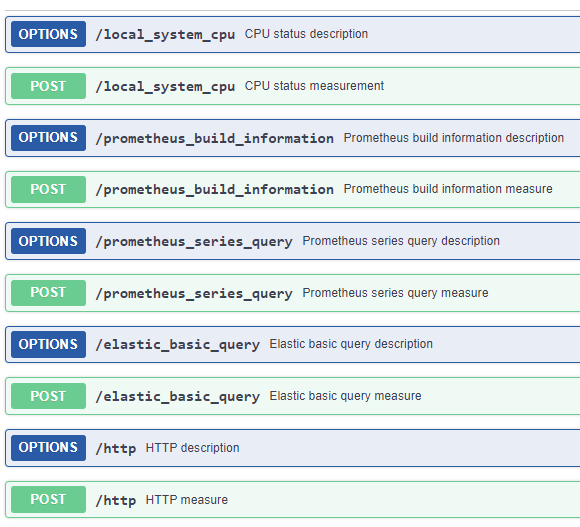
\includegraphics[width=.8\linewidth]{images/swagger/swagger_UI_API.png}
	\caption[Interfaccia di Swagger API esposte]{Interfaccia di Swagger contenente tutte le \gls{API} esposte }\label{swagger ui options/post}
\end{figure}

Andando ad interagire con l'interfacci proposta è possibile, tramite il menù a tendina, espandere la singola \gls{API} vedendone i relativi dettagli.
La Figura \ref{swagger ui post} mostra come deve essere costruito il body di una richiesta di quel tipo, andando a fornire un esempio di valori per quello specifico Schema.
Tramite il bottone ``\textit{Try it out}'' è possibile inviare una richiesta personalizzata su quello specifico endpoint.

\begin{figure}[htb]
	\centering
	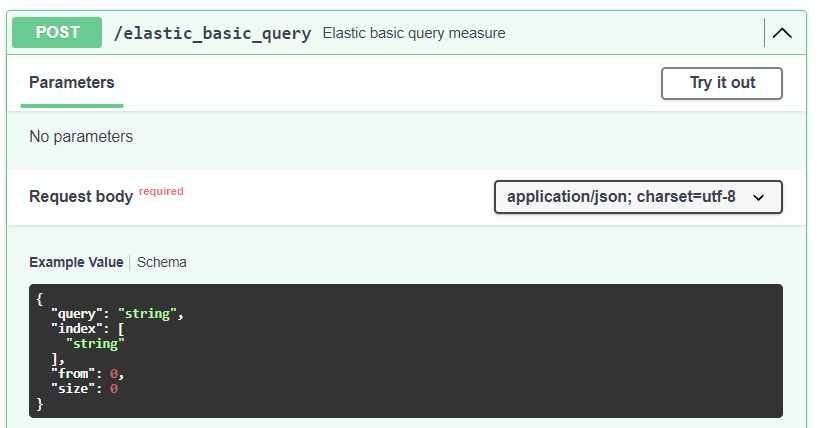
\includegraphics[width=.8\linewidth,]{images/swagger/swagger_UI_post.png}
	\caption[Interfaccia di Swagger esempio richieste POST]{Interfaccia di Swagger contenente un esempio di schema per richieste Post }\label{swagger ui post}
\end{figure}

Si possono ottenere maggiori dettagli riguardo la struttura consultando la sezione Schema, come mostrato nella Figura~\ref{swagger ui schema}, che fornisce anche il tipo associato ai campi.

\begin{figure}[htb]
	\centering
	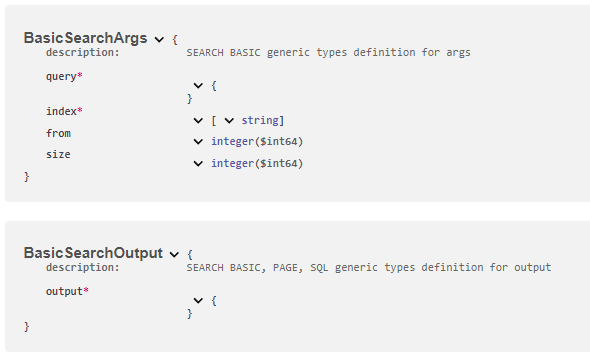
\includegraphics[width=.8\linewidth]{images/swagger/swagger_UI_schema.png}
	\caption[Interfaccia di Swagger schema json con i tipi associati ai valori]{Interfaccia di Swagger contenente lo schema json con i tipi dei valori}\label{swagger ui schema}
\end{figure}


La Figura \ref{swagger ui post response} mostra invece le possibili risposte, con i relativi \textit{status code}, che si possono ottenere inviando una richiesta su uno specifico endpoint; viene anche qui specificato lo schema della risposta in formato JSON.

\begin{figure}[htb]
	\centering
	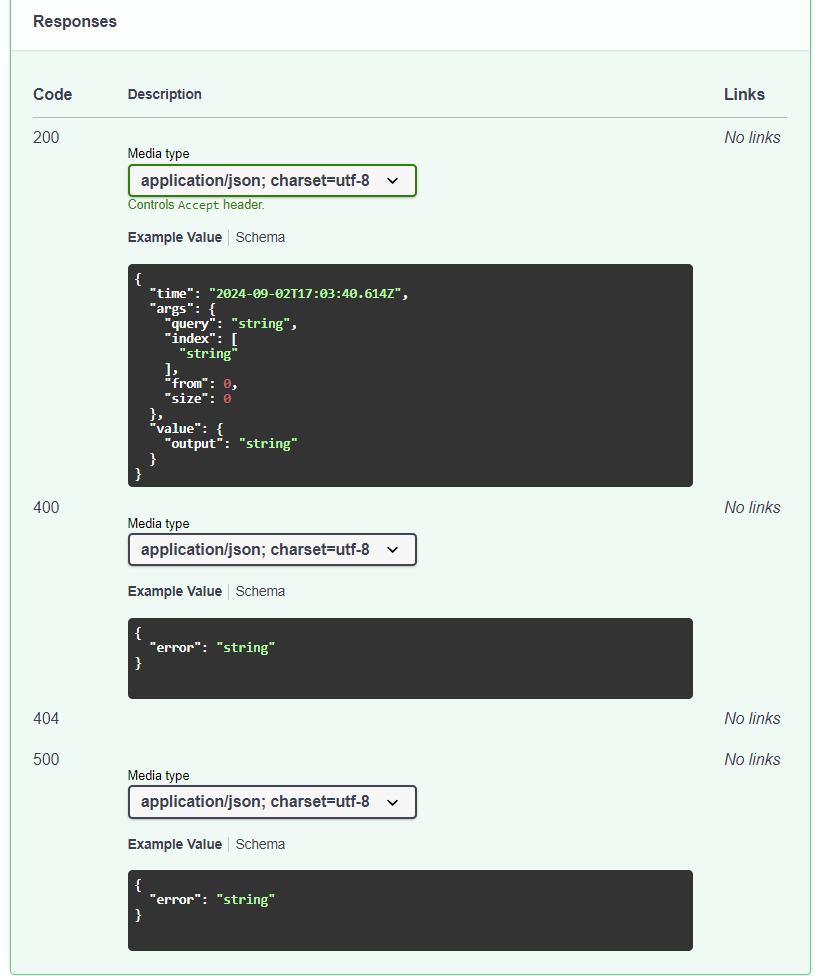
\includegraphics[width=.8\linewidth]{images/swagger/swagger_UI_response.png}
	\caption[Interfaccia di Swagger schema risposte POST]{Interfaccia di Swagger contenente lo schema delle risposte alle richieste POST}\label{swagger ui post response}
\end{figure}


\subsection{Deployment e Vantaggi}\label{vantaggi scal rep}
L'\textit{Assurance Engine} è stato progettato per essere eseguito all'interno di un cluster kubernetes, sfruttando la containerizzazione per garantire una distribuzione semplice e flessibile.
In particolare, l'applicazione viene impacchettata in un container Docker (docker image) minimale contenente il binario eseguibile dell'engine che successivamente viene deployato all'interno del cluster Kubernetes.
Una volta in esecuzione all'interno del cluster, l'applicativo cercherà di collegarsi agli altri servizi integrati nell'engine e disponibili all'interno dell'ecosistema, come Elasticsearch o Prometheus ad esempio. \\
Il sistema, per come è strutturato, si pone da \emph{intermediario} tra l'utente finale e alcuni servizi di monitoring facendo in modo di ricevere le richieste dall'utente e successivamente indirizzarle all'apposito servizio. Questa infrastruttura può essere vista in un certo senso come un \textit{request-reflector} che però, adottando questo design di sviluppo, fornisce svariati vantaggi tra cui la garanzia di alcune proprietà chiave per l'Assurance Engine, come la \emph{scalabilità}, la \emph{replicabilità} e l'\emph{assenza di coordinazione aggiuntiva} in ambienti distribuiti.

\paragraph{Scalabilità e Replicabilità}
Queste importanti proprietà, derivanti dalla struttura dell'applicazione, consentono di deployare l'engine come una singola istanza o come istanze multiple, permettendo quindi di scegliere il numero di \emph{repliche deployabili} per rendere il sistema distribuito. \\
L'architettura, pur essendo distribuita, non necessita alcuna coordinazione aggiuntiva tra le varie istanze/repliche in quanto tutte \emph{equivalenti e intercambiabili} tra loro: le richieste possono essere inviate indistintamente a una qualsiasi istanza disponibile e verranno risolte in modo identico. Un \emph{network load balancer}, come un \emph{kubernetes service}, si occuperà di distribuire il traffico, in base alle condizioni della rete, tra le varie repliche disponibili.
Questa semplicità è possibile perché il compito che ogni replica assolve è quello di intermediario \textit{stateless} verso servizi di backend come Elasticsearch. \\
La Figura \ref{assurance engine deployment} mostra uno schema di un semplice cluster in cui sono state deployate 3 repliche dell'Assurance Engine poste dietro ad un network load balancer.
Indipendentemente dalla replica a cui la richiesta verrà inoltrata dal load balancer, esse arriveranno sempre allo stesso servizio di backend.

\begin{figure}[h!]
	\centering
	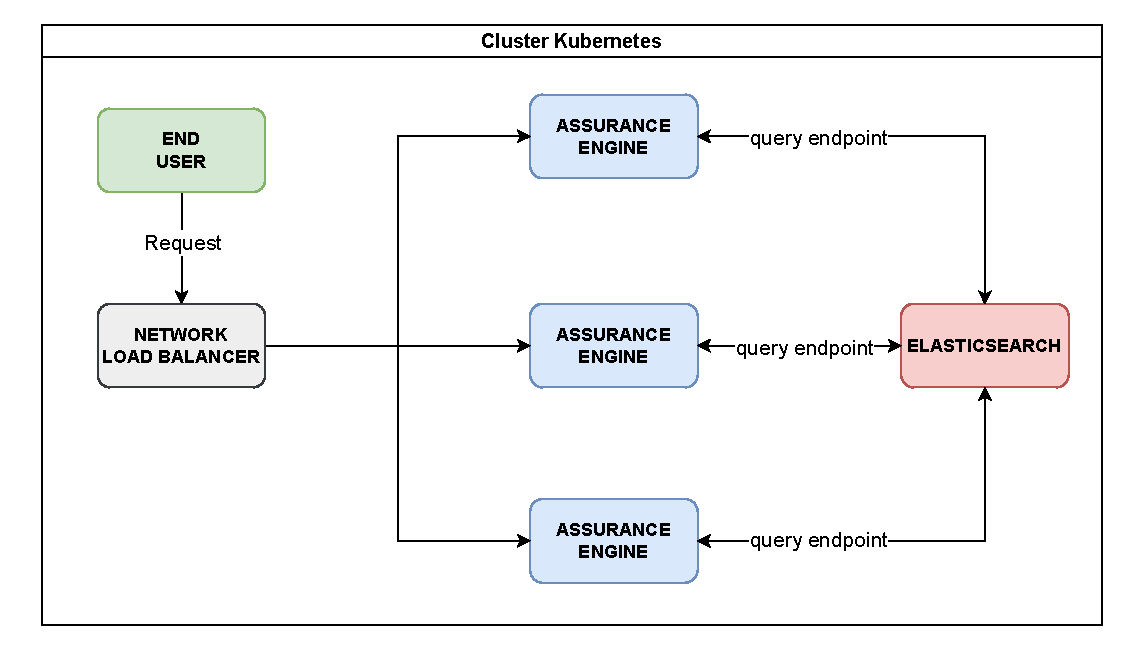
\includegraphics[width=.9\linewidth]{images/ae/AssuranceEngine.drawio.pdf}
	\caption{Diagramma Assurance Engine deployato su 3 nodi}\label{assurance engine deployment}
\end{figure}

\subsubsection{Necessità di questo ''framework intermediario''}
Lo scopo di un sistema di assurance è garantire il soddisfacimento di determinate proprietà da parte di un sistema target. \\
La domanda che viene spontaneo porsi è quindi:
\textit{Come mai, essendo che Elasticsearch fornisce analisi per informazioni provenienti da una moltitudine di entità diverse, si è ricorsi ad un layer aggiuntivo (assurance engine), posto tra l'utente e il servizio di backend, per svolgere controlli di assurance?} \\
La risposta a questa domanda si trova nella definizione di sistema di assurance posta qua sopra; un sistema di assurance è quanto più completo e generico quante più proprietà e sistemi target eterogenei riesce a verificare. \\
Aggiungendo questo strato di interfacciamento è stato possibile accaparrarsi tutti i \textbf{vantaggi di Elasticsearch}, come la possibilità di collezionare dati da una moltitudine di servizi eterogenei grazie alle specifiche \textit{Integration} e l'\textit{efficienza} nel salvataggio e nella ricerca dei dati in un sistema distribuito.
A questi, vanno ad aggiungersi i \emph{vantaggi architetturali dell'assurance engine} illustrati nella Sezione precedente \ref{vantaggi scal rep}, che garantiscono \textbf{scalabilità} e \textbf{replicabilità}.
Infine, il punto chiave che giustifica questo strato, si riconduce alle potenzialità che vengono offerte dall'utilizzo di un \textbf{linguaggio di programmazione} efficiente e affidabile come Rust.
Utilizzando un vero e proprio linguaggio di programmazione invece che il limitato linguaggio di scripting \textit{built-in} di Elasticsearch, è possibile avere una potenza espressiva maggiore sia per fare controlli più complessi (contratti) che per ottenere dati in modalità non implementate nei servizi di backend (\textit{probe custom}). Alcuni esempi sono l'invio di semplici richieste HTTP verso un sito web per verificarne l'availability oppure l'invio di payload specifici su determinati endpoint per monitorarne la reazione; questo tipo di attività, possibile grazie all'impiego di un linguaggio di programmazione, permette quindi di analizzare contesti più generici.
I servizi come Elasticsearch, invece, non consentono l'invio di richieste avanzate o \textit{taylor-made} verso target specifici; il servizio recupera delle metriche dal target ma non ha una parte di ''\textit{probe custom}'' che gli permette di ottenere informazioni specifiche. \\
In conclusione il vantaggio si piò riassumere in una parola \textbf{genericità}, si possono combinare informazioni da varie entità diverse.


\subsection{Funzionamento}\label{funzionamento ae}
Viene illustrato un esempio di ciclo completo di funzionamento.
La Figura \ref{assurance engine flow} mostra un'automa a stati finiti contenente lo schema del funzionamento illustrato tramite componenti grafici.

\begin{figure}[ht!]
	\centering
	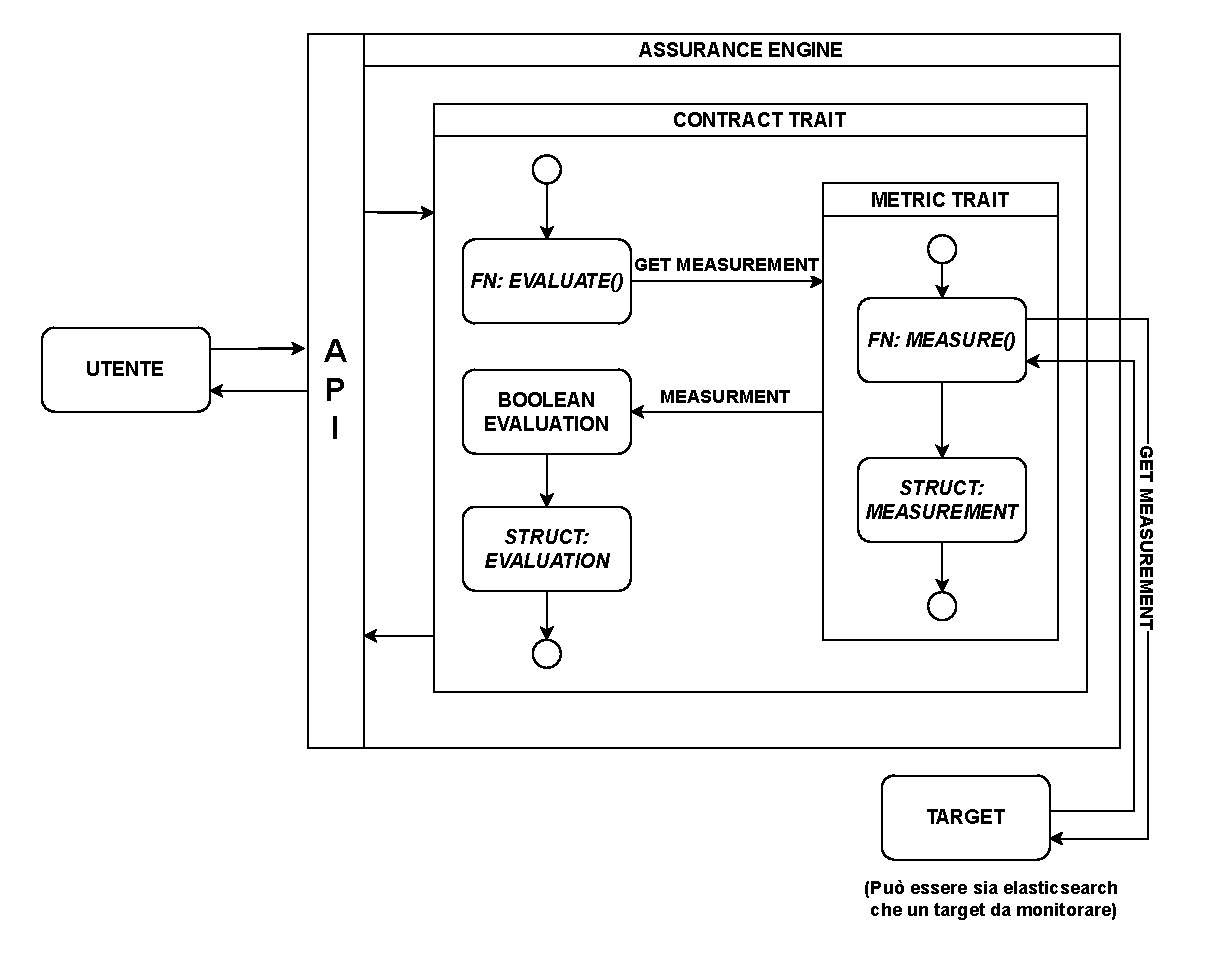
\includegraphics[width=.9\linewidth]{images/ae/Assurance_engine_flow.drawio.pdf}
	\caption{Assurance Engine: Flusso di esecuzione}\label{assurance engine flow}
\end{figure}

La prima operazione inizia dall'utente che invia una richiesta ad un endpoint esposto dal'\textit{Assurance Engine}, supponiamo per completezza il metodo POST di un contratto.
Il server, quando riceve la richiesta, va ad eseguire il metodo \texttt{evaluate()} definito per quella funzionalità. L'esecuzione può essere suddivisa concettualmente nelle 3 parti focali precedentemente definite nell'\emph{Assurance Process} definito nella Sezione \ref{assurance process}; rispettivamente sono \emph{Measurement collection}, \emph{Contract evaluation} e {Report composition}.

\paragraph{Measurement collection}
In questa fase viene eseguito il metodo \texttt{measure()} precedentemente illustrato nella Sezione \ref{metric trait} che si occupa di ottenere delle metriche da un target. Come accennato prima, grazie alla genericità di cui gode, il metodo \texttt{measure()} può andare ad interrogare un servizio di backend come Elasticsearch o inviare richieste custom.
I dati ottenuti vengono trattati come \texttt{measurements} e di fatto costituiscono le \textit{evidence} o prove necessarie ai contratti per stilare una valutazione del sistema; seguono il modello definito nella Sezione \ref{measurement section}.
Viene effettuata quindi una fase di parsing della risposta JSON ottenuta all'interno del \textit{measurement} andando ad estrarre i campi e i valori desiderati; vengono svolte anche operazioni di aggregazione dei dati come somme, medie, ecc (\emph{metric evaluation}).
Una volta ottenute le evidence definitive inizia la seconda fase.

\paragraph{Contract evaluation}
Questa fase è concettualmente molto semplice ma racchiude al suo interno la potenzialità e le garanzie che questo sistema può offrire. Si tratta di controlli booleani effettuati tra le \emph{measurements} ottenute facendo \emph{metric evaluation} e gli argomenti passati come parametri al contratto, precedentemente visti nella Sezione \ref{contract section} alla Figura \ref{argument contract struct}.
I risultati dei vari controlli singoli sulle metriche vengono successivamente aggregati in un'unico risultato finale che dichiara il soddisfacimento o meno della proprietà che si stava verificando.

\paragraph{Report composition}
L'ultima fase si tratta semplicemente di ritornare i risultati ottenuti in modo formale e valutabile a posteriori. Viene quindi ritornata la struttura definita nella Sezione \ref{evaluation section} contenente sia l'esito che gli argomenti usati per fare la valutazione, in aggiunta al \textit{timestamp}.

L'utente che ha inviato la richiesta riceve una risposta in formato JSON, contenente o la struttura sopra definita oppure una descrizione della tipologia dell'errore che è incorso.


\subsection{Esempi di richieste: Elastic e SQL Query}
Di seguito vengono proposti tre esempi di utilizzo del metodo \texttt{measure()}, per raccogliere metriche da Elasticsearch, con tre query differenti in formato JSON. Le prime due sfruttano il linguaggio di ricerca fornito da Elasticsearch, un completo Query \gls{DSL} basato su JSON, mentre la seconda permette di effettuare ricerche usando query SQL e ritornando i risultati in forma tabellare. \\
L'ultimo esempio mostra uno schema generale di invocazione del metodo \texttt{measure()} con una generica query.

\begin{exmp}
	Esempio di ricerca che colleziona \textbf{tutti i dati} presenti nell'indice e li ordina cronologicamente sulla base dei campi Date e Time del dataset. Di seguito, nel Codice \ref{JSON query all}, viene mostrata la query in formato JSON necessaria per svolgere tale operazione.

	\begin{lstlisting}[language=json, caption=Valori JSON per query \emph{match all} \label{JSON query all}, basicstyle=\ttfamily]
  "query": {
      "match_all": {}
      },
  "sort": [
      {"Date": {"order" : "asc"}},
      {"Time": {"order" : "asc"}}
  ],
  \end{lstlisting}
\end{exmp}

\begin{exmp}
	Esempio di ricerca che colleziona i dati presenti nell'indice il cui \textbf{intervallo temporale}, campi Date e Time, rispetta un certo criterio e li ordina cronologicamente. Di seguito, nel Codice \ref{JSON query range}, viene mostrata la query in formato JSON necessaria per svolgere tale operazione.

	\begin{lstlisting}[language=json, caption= Valori JSON per query \emph{range} su intervalli temporali \label{JSON query range}, basicstyle=\ttfamily]
  "query": {
    "range": {
        "Date": {
            "gte": "11/03/2004",
            "lte": "15/03/2004"
        },
        "Time": {
            "gte": "18.00.00",
            "lte": "24.00.00"
        }
    }
  },
  "sort": [
      {"Date": {"order" : "asc"}},
      {"Time": {"order" : "asc"}}
  ],
  \end{lstlisting}
\end{exmp}

\begin{exmp}
	Esempio di ricerca eseguito tramite query \textbf{SQL} che estrae due campi dall'indice filtrando per il campo Date. Nel Codice \ref{JSON query sql}, viene mostrata la query in formato JSON necessaria per svolgere tale operazione.

	\begin{lstlisting}[language=json, caption= Valori JSON per query \emph{SQL} \label{JSON query sql}, basicstyle=\ttfamily]
    "query": "SELECT T, \"NO2(GT)\"
              FROM imported_dataset
              WHERE Date = '05/10/2004'"
  \end{lstlisting}
\end{exmp}


\begin{exmp}
	Nel seguente Codice \ref{rust query} viene mostrata l'invocazione del metodo \texttt{measure()} con la relativa generica query specificabile tramite valori JSON nel Query \gls{DSL} di Elastic.

	\begin{lstlisting}[language=rust, caption= Esecuzione Rust della query nel linguaggio di Elastic\label{rust query}, basicstyle=\ttfamily]
  client.measure(BasicSearchArgs {
      query: json!({<json_values>}),
      index: vec!["imported_dataset".to_string()],
      from: None,
      // size: Some(1)
      size: None,
  })
  \end{lstlisting}

	Mentre in questo Codice \ref{rust query sql} viene mostrata l'invocazione del metodo \texttt{measure()} con la relativa generica query SQL specificabile tramite valori JSON.
	\begin{lstlisting}[language=rust, caption= Esecuzione Rust della query SQL \label{rust query sql}, basicstyle=\ttfamily]
  client.measure(ArgsSQL {
    query: json!({<json_values>})
  })
  \end{lstlisting}
\end{exmp}

% OPTIONAL TODO
%\subsection{Dettagli extra - opzionale}
%%+ forse dettagli tokio o in una subsection
%\hl{
%	Dettagli implementativi extra: \\
%	-ambiente asincrono (tokio) che distribuisce il carico (valutazione %metriche, contratti, ecc) in modo efficacemente su più core (asincrono %run time work stealing, scala bene su più core)\\
%}
